% !TeX program = lualatex
% Frequency or wavelength spectrum of a laser pulse when compressed in the CPA technique
% Autor: Ismael Torres García
\documentclass[tikz,border=8pt]{standalone}
\usetikzlibrary{calc}
\usepackage{pgfplots}
\pgfplotsset{
    compat=1.9,
    colormap={spectrum}{
        color(0.00000000000000bp)=(violet); 
        color(8.33333333333333bp)=(blue);
        color(16.66666666666670bp)=(cyan);
        color(25.00000000000000bp)=(green);
        color(33.33333333333330bp)=(yellow);
        color(41.66666666666670bp)=(orange); 
        color(50.00000000000000bp)=(red)
    }
}
\begin{document}

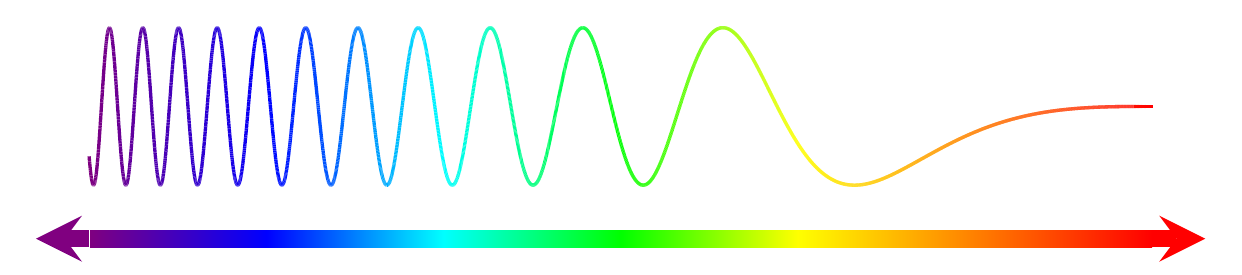
\begin{tikzpicture}[x=3cm, y=1cm] % las unidades de tikz

\begin{axis}[
  % para pgfplot utilice las mismas unidades que tikz
  x=3cm, y=1cm,
  % dominio de la función
  domain=-4.5:0,
  % enseñar solo el dominio
  xmin=-4.5, xmax=0,
  % no enseñar los salientes de los ejes
  axis lines=none,
  % define el mapa de colores, azul-rojo invertido
  colormap name=spectrum,
  % si usas 'rel axis cs', añade la línea de abajo para mostrar los contenidos del eje
  clip=false,
  % colorbar propiedades
  colorbar horizontal,
  colorbar style = {
    at = {(0, -0.20)},
    height=6pt,
    anchor=west,
    axis lines=none,
    % ticks=none,
  }
]
\addplot[
  mesh, point meta=x,
  % muestras
  samples=5000,
  line width=1.2pt,
]{
  % la función senoidal
  sin(45*x^3)
};

% flechas en los extremos de la barra de colores
\draw[->, >=stealth,line width=6pt, anchor=east, color=violet] 
(rel axis cs: 0, -0.20) -- (rel axis cs: -0.05, -0.20);
\draw[->, >=stealth,line width=6pt, anchor=west, color=red] 
(rel axis cs: 1, -0.20) -- (rel axis cs: 1.05, -0.20);

\end{axis}
\end{tikzpicture}

\end{document}
